\startchapter{Software Implementation}
\label{chapter:implementation}
\section{Introduction}
The \Name was build to be a stand-alone application.
In order to allow it to be a powerful yet simple application the technologies used were selected with the idea of portability in mind.

\section{Technologies Used}
\subsection{\Xilinx}
\Xilinx is one of the two largest manufacturers of \acrshort{FPGA}s. 
Their devices are considerably more popular than their competitors.
The configuration of devices employs a well known series of steps referred to as the \Xilinx 'tool-chain'~\cite{xilnxDevManual}.
The 'tool-chain' not only compiles user designs and constraints into the configuration \gls{Bitstream} but performs a series of complex operations to optimize designs and effectively implement them on any \Xilinx model of the user's choosing.
\begin{enumerate}
	\item \textbf{\gls{sch2hdl}}: \glsdesc{sch2hdl}
	\item \textbf{\gls{XST}}: \glsdesc{XST}
	\item \textbf{\gls{MAP}}: \glsdesc{MAP}
	\item \textbf{\gls{PAR}}: \glsdesc{PAR}
	\item \textbf{\gls{ngdbuild}}: \glsdesc{ngdbuild}
	\item \textbf{\gls{trce}}: \glsdesc{trce}
	\item \textbf{\gls{Bitgen}}: \glsdesc{Bitgen}
\end{enumerate}
Each step produces a series of files that are used for a variety of purposes. 
Often the resultant files are used by the subsequent step but some are intended for user information.
The \gls{ngdbuild} tool generates what is known as the netlist for the design.
The netlist is a description of the connectivity of the circuit implemented on the device. 
The generated netlist is in a non human-readable format in an 'ndc' file.
Fortunately, \Xilinx provides an additional tool called \acrshort{xdl2ndc} which allows the conversion to the human-readable \acrfull{XDL}.
\subsubsection{\acrfull{XDL}}
The \acrfull{XDL} is a human-readable ASCII format; though it is not actively part of the 'tool-chain' it is considered a native netlist format for describing and representing \acrshort{FPGA} designs~\cite{xdlTutorial}. 
A part is a human-defined component which is to be implemented.
Netlists either contain or refer to descriptions of the parts used and where in the device they are implemented.
When a part is used it is called an 'instance'; thus each 'instance' has a definition, sometimes referred to as a master.

An \acrshort{XDL} file contains two sections, the instance placement and configuration section, and the net routing section. 
The placement and configuration section provides a list of every instance in a design. 
Their descriptions include all of the configuration details required for their implementation on a component (power settings, logic, timing configurations... etc).
In the \Xilinx jargon, a net refers to any electrical path between two components; more specifically, a net describes a communication channel.
The gate-array of a \Xilinx device is composed of a grid of wires.
These wires can be fused together by \acrfull{PIP} to make a useful connection between two components, thus creating a net.
The output-pin of a net receives the signal from the transmitting component while the input-pin delivers the signal to the receiver.
The \acrshort{PIP}s in-between dictate the path the signal takes between the two components.
The net routing section of the \acrshort{XDL} file describes every path in the design.
Combined, these two sections completely describe a design and how it is implemented.
\subsubsection{XDLRC} \label{sec:XDLRC}
The \acrshort{XDL} file describes the design implemented on a device.
From this a lot of information regarding the composition of a \Xilinx device can be learned but it does not provide the entire description; only what has been used by the design.
The \acrshort{xdl2ndc} command line tool provides an option to generate a resource report file referred to as an XDLRC file. 
A XDLRC file describes the entire architecture of a \Xilinx \acrshort{FPGA}.
\ConditionSize
\begin{lstlisting}[label={lst:xdlrc}, language=Python, caption={A hierarchical XDLRC resource description of a Spartan 6 FPGA consisting of a header, a tile section, and a trailing device summary~\cite{xdlTutorial}}]
#Header section
(xdl_resource_report v0.2 xc6slx16csg324-3 spartan6
# Device Level Dimensions
(tiles 73 62
...
	#Configurable logic block with two slices
	(tile 4 6 CLEXL_X1Y61 CLEXL 2
		(primitive_site SLICE_X0Y61 SLICEL internal 45
			(pinwire A1 input L_A1)
		...
		(primitive_site SLICE_X1Y61 SLICEX internal 43
		...
		(pinwire D output XX_D)
	...)
	# Interconnect tile
	(tile 4 5 INT_X1Y61 INT 1
	...
		(wire EE2B0 2
			(conn CLEXM_X2Y61 CLEXM_EE2M0)
			(conn INT_BRAM_X3Y61 EE2E0)
		...
		# Programmable Interconnect Points
		(pip INT_X1Y61 EE2E0 -> EE2B0)
		(pip INT_X1Y61 EE4E0 -> EE2B0)
		(pip INT_X1Y61 EL1E_S0 -> LOGICIN_B9)
	...)
# summary
(summary tiles=4526 sites=5378 sitedefs=46 numpins=157962 numpips=5782505))
\end{lstlisting}
\normalsize

Listing~\ref{lst:xdlrc} provides and example of the XDLRC format.
The report begins with a header describing the device.
It then reports that the overall architecture contains a matrix of tiles 73-wide and 62-tall.
Further down we can see a configurable logic block at coordinate (4,6) and an interconnect tile at coordinate (4,5) are shown.
Each of these tile descriptions provide details of the subcomponents they contain, pinwires, \acrshort{PIP}s, slices...etc.
The tool is capable of generating a variety of different XDLRC files for a device, ranging in the level of detail.
The smaller files can range around 10MB while the fully detailed descriptions can reach 7GB.
\subsection{Java} \label{sec:java}
Java is a powerful and general-purpose programming language. 
It is specifically designed to be as independent as possible.
The original developer, James Gosling, intended the language to allow developers a comfortable implementation experience with seamless deployment. 
The custodians of the Java language, Sun Microsystems, promotes the slogan 'write-once, run anywhere'.  
\Name was written in Java primarily in order to interface with the \acrshort{API} known as \RapidSmith which is described in section~\ref{sec:rapidSmith}.
However, the additional benefits of allowing \Name to be compact, cross-platform application can not be understated.
The Java language provides a native \acrfull{GUI} toolkit known as \Swing.
\Swing is an \acrshort{API} that is part of Oracle's Java Foundation Classes; in other words it is readily available to all users of Java.
It provides a simple to use programming structure for creating sophisticated \acrshort{UIs}.
\Name employs Java and Java \Swing to make it as user-friendly as possible. 

\subsection{\RapidSmith} \label{sec:rapidSmith}
\RapidSmith is a set of tools and \acrfull{APIs} written in Java that enable \acrfull{CAD} tool creation for \Xilinx \acrshort{FPGA}s~\cite{rapidSmith}.
Its purpose is to be used as a rapid prototyping platform for experimentation and research.
The code is freely to use readily accessible.
It was chosen as a supporting library for \Name for several reasons.
First, the code base provides a series of class structures that astutely mirrors structure of \Xilinx devices and infrastructure.
Secondly, it provides ready-made tools for extracting frames \gls{Bitstream} files. 
\gls{Bitstream} files are huge binary files, without the tools provided by \RapidSmith the analysis of these files becomes an arduous task.
Finally, and most importantly, the creators of \RapidSmith have developed a means of condensing XDLRC files into a greatly compressed format referred to as a 'database' file.
\Name requires considerable detail of an \acrshort{FPGA}'s architecture in order to accurately described the effects a trojan has on a design.
As mentioned in section~\ref{sec:XDLRC}, the fully detailed XDLRC files can reach 7GB in size.
Working with text-based files of this size determents performance to an unusable level.
The makers of \RapidSmith have developed a compression scheme which converts the XDLRC files into a non human-readable format.
The compression scheme reduces the size of the XDLRC files from 7GB to 1.3MB. 
The \acrshort{API} provides interface classes that support querying the compressed files.
With these features \RapidSmith enables the ability to analyze the effect any discovered trojan has on a device.
\subsubsection{Class Structure} \label{sec:classStructure}
Building off of the information provided by the XDLRC architecture files, \RapidSmith provides a class structure that enables developers an easy to use interface for working with \acrshort{FPGA}s.
As described in section~\ref{sec:architectureAndConfig}, the gate-array of an \acrshort{FPGA} is composed of blocks made up of tiles.
These tiles are further composed of sub-components collectively referred to as 'primitives'.
Figure~\ref{fig:classStructures} shows the top-down construction of the \RapidSmith class structure.
The \Name employs both the 'Device' and 'Design' classes shown in Figures~\ref{fig:rapidSmithDevice} and~\ref{fig:rapidSmithDesign} respectively.
The \gls{Bitstream} for the \gls{golden} and \gls{target} devices are read into memory. 
The \gls{Bitstream} parser class determines the model of the devices and the 'Device' class is then loaded.
When loaded the 'Device' class imports the compressed XDLRC file describing the chosen model.
The complete description of the architecture is read and loaded; every tile, primitive, wire, and how they all interconnect is stored in memory.
The \gls{golden} \acrshort{XDL} file is then loaded.
The \acrshort{XDL} files is read and the 'Design' class is similarly loaded with the user-defined design.
\begin{figure*}[h]
	\centering
	\begin{subfigure}[t]{0.5\textwidth}
			\centering
			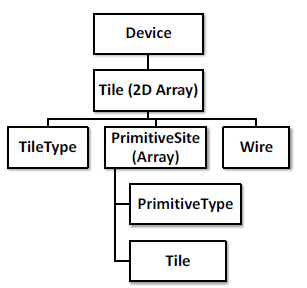
\includegraphics[height=2in]{Figures/rapidSmithDevice}
			\caption{The Device Class-Structure}
			\label{fig:rapidSmithDevice}
	\end{subfigure}%
	~ 
	\begin{subfigure}[t]{0.5\textwidth}
		\centering
		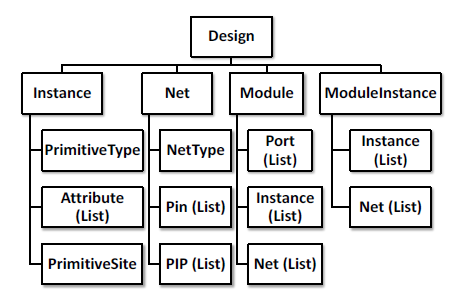
\includegraphics[height=2in]{Figures/rapidSmithDesign}
		\caption{The Design Class-Structure}
		 \label{fig:rapidSmithDesign}
	\end{subfigure}
	\caption{The \RapidSmith Class Hierarchy~\cite{rapidSmithManual}}
	 \label{fig:classStructures}
\end{figure*}
Not shown in Figure~\ref{fig:classStructures} are a series of utility classes.
The \gls{Bitstream} parser class reads and interprets the \gls{Bitstream} files. 
It uses a 'Frame' class to organize the \gls{Bitstream} file into an array of objects that adhere to the configuration pattern described in section~\ref{sec:architectureAndConfig}.
The frame objects are populated with the frame's 32-bit address, an array of 32-bit words which make up the frame and a series of helper methods.
\section{Design}
\subsection{\acrfull{UI}}
\begin{figure}
\centering
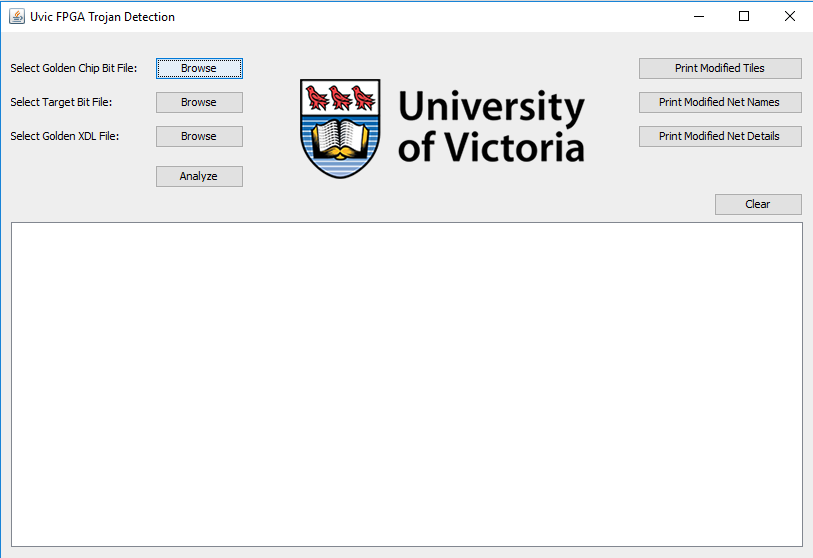
\includegraphics[width=0.7\linewidth]{Figures/UI}
\caption[The User-Interface of the \Name]{The User-Interface of the \Name}
\label{fig:UI}
\end{figure}

\subsection{Operation}
\subsection{Use-Manual}
